\textbf{\bfseries Christian Limbert Paredes Aguilera}\\
\textbf{Análisis de decisiones económicas}\\\\
\subsection*{\center TAREA 4}
\vspace{.4cm}
\subsection*{\center POLÍTICAS PÚBLICAS}
\vspace{1cm}


\begin{enumerate}[\bfseries 1.]

    % ---------- 1.
    \item Tome en cuenta, los países de Noruega, EEUU y Brasil esto según fuente de datos PovcalNet en internet: http://iresearch.worldbank.org/PovcalNet/home.aspx\\\\  
	\begin{center}
	\texbf{\Large \bfseries Curva de Lorenz}\\\\
	    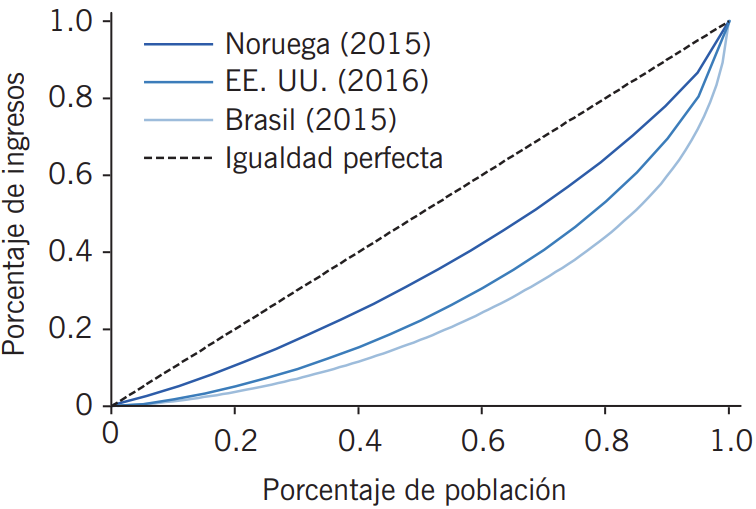
\includegraphics[scale=.35]{codigoFuente/tareas/decisiones/image/gini.png}
	\end{center}
	\vspace{.7cm}
    Si una de las curvas de Lorenz se encuentra debajo de otra, la distribución  es más desigual que la otra. Por lo tanto está claro que en la figura Noruega el más igualitario y Brasil el más desigual de los tres.\\
    El índice de Gini es el área entre la curva de Lorenz y la línea de igualdad perfecta, sobre el área total debajo de dicha linea. Ya que es un índice o coeficiente sus valores se encuentra entre 0 igualdad perfecta y 1 (Sólo una persona obtendría los ingresos de los demás), en consecuencia cuanto menor es el valor de Gini, más igualitaria es una sociedad. 
    Según (https://data.oecd.org/inequality/income-inequality.htm) Noruega tiene un índice de 0,27, donde podemos considerar de baja desigualdad, contrariamente a Brasil(2013) con un 0.5. Cabe mencionar que las economías con valores de Gini superiores a 0,5 se consideran muy desiguales este podría ser el caso de Bolivia,  Colombia o Zambia. \\
    Cabe mencionarse que EEUU(2013-2019) se mantuvo con un indice constante y noruega tuvo una alza de desigualdad desde 2014 para adelante.\\\\ 

    % ---------- 2.
    \item  Para el caso de Noruega el sistema tributario se tiene un taza fija aplicable, y una parte progresiva en función a los ingresos. El tipo fijo del impuesto de la renta es del $22\%$. Además, para aquellos cuya base imponible supere las 184.800 coronas (18.480€) anuales, también se aplicará un tipo progresivo.\\\\
    Con respecto a programas de mantenimiento de los ingresos, las mujeres tienen derecho a una baja por maternidad de 46 semanas (cobrando el $100\%$ del salario) y los hombres disponen de 10 semanas de permiso cobrando el $100\%$ de su salario. Por otro lado Las personas desempleadas tienen derecho a cobrar la prestación por desempleo siempre que hayan cobrado menos de $17.000$ dolares aproximadamente en el año anterior o bien menos de unos 34.000 dolares en los tres últimos años. La cantidad a cobrar como prestación es de cerca del $85\%$ de su salario y su duración es de $500$ días.\\\\

    Y con respecto a subsidios a los servicios públicos, el sistema educativo en todos sus niveles es prácticamente gratuito y obligatorio. El sistema de salud es sólo gratuita para menores de 16 años y para mujeres embarazadas y en periodo de lactancia, luego todos deben pagar una cuota anual de 222 dolares que te da derecho a asistencia gratuita durante el resto del año. Los hospitales públicos son gestionados por cuatro Autoridades Sanitarias Regionales, que son supervisadas por el Ministerio de Sanidad y Servicios Asistenciales.




\end{enumerate}

